\documentclass[12pt,a4paper]{article}	%es gibt noch andere Arten of course, wie book zB, aber mit article kommst du gut hin
\usepackage[utf8]{inputenc}
\usepackage[german, english]{babel} 
\usepackage[T1]{fontenc}
\usepackage{amsmath}
\usepackage{bm}
\usepackage{mathtools}

\usepackage{amsfonts}
\usepackage{amssymb}
\usepackage{makeidx}
%\usepackage{esvect}
\usepackage{hyperref}
\usepackage{amsmath}
\usepackage{listings}
\usepackage{subfigure}		%nützlich, wenn du mehrere Bilder in eine Bildumgebung packen möchtest
\usepackage{tabularx}		%für tabellen
\usepackage{chngcntr}
\counterwithin{equation}{section}	%damit Gleichung pro section durchgezählt werden und nicht insgesamt
\counterwithin{figure}{section}		%das gleiche für Bilder
\usepackage{graphicx}
%\usepackage{stackengine}
\usepackage[left=3cm,right=3cm,top=3cm,bottom=3cm]{geometry}
\usepackage[singlespacing]{setspace}	%macht einziligen Zeilenabstand. ansonsten onehalfspacing oder doublespacing

\newcommand{\etan}{\eta_{0}}
\newcommand{\R}{\vv{R}=X\vv{e_{x}}+Y\vv{e_{y}}}
\newcommand{\phid}{\dot{\phi}}
\newcommand{\Yd}{\dot{Y}}
\newcommand{\Xd}{\dot{X}}
\newcommand{\F}{\mathcal{F}}
\newcommand{\p}{\mathcal{P}}
\newcommand{\x}{\textbf}
\newcommand{\norm}[1]{\left\lVert#1\right\rVert}
\newcommand{\abs}[1]{\left\lvert#1\right\rvert}

\begin{document}
%\setcounter{section}{2}

\setlength{\parindent}{0pt}


\thispagestyle{empty}

\begin{titlepage}
	\centering
	
\includegraphics[width=0.45\textwidth]{logo_sw.jpg}\par\vspace{1cm}
	\vspace{1cm}
%	{\scshape\Large Spezialisierung\par}
	\vspace{1.5cm}
%	{\LARGE\bfseries working title\\wedge confinement in LC systems  \par}
	{\LARGE\bfseries Assignment Sheet Nr. 5\\  \par}
	\vspace{1cm}
	
	{\large	Paul Monderkamp, Matr.Nr. 2321677\par}
	\vfill
	

	\vfill

% Bottom of the page
	{\large  monderkamp@thphy.uni-duesseldorf.de \par}
	\vspace{2cm}
	%{\large Abgabedatum: 00.04.2017 \par}
\end{titlepage}

\thispagestyle{empty} %macht dass da keine Seitennummer drauf ist.
\newpage	%beendet die Seite und macht auf der nächsten weiter

%\section*{Abstract}
%
%The aim of this specialization report is to summarize the fundamental concepts that are necessary to understand the physical properties of liquid crystal systems and their formation.\\
%The final objective for the masters thesis is to investigate the phase behaviour of those systems in confined space. As a step towards this goal, the algorithm that is used for this problem is introduced and explained. To verify its validity one section of this report is dedicated to recreation of phase behaviour predicted by previous publications on the subject of liquid crystals such as those in this report.\\
%The derivation of the algorithm that is used to generate the corresponding results uses geometrical concepts to guarantee meaningful predictions about the relative positions of the molecules that make up the systems in this thesis. \\
%Beyond that all results are generated via numerical methods. The programming languages used in this thesis are \x{C}/\x{C++} for the generation of the numerical results and \x{MatLab} for the evaluation, processing and visualization of the data. 

%The aim of this bachelors thesis is to provide an overview over the most fundamental theoretical principles which form the basis for the \x{Theory of viscotaxis of microswimmers}. Exemplary geometries of swimming particles are chosen that successively illustrate phenomena typical of the behaviour of systems under the influence of this theory.\\
%Every section which deals with the investigation of a single statement of a problem is divided into two subsections. The first section gives the equations of motion and the respective solutions, and the second one explains the solutions in a physical context and discusses the implications. \\
%All results are purely achieved by analytical methods presented in the respective sections. 

%\newpage


\tableofcontents %macht ein Inhaltsverzeichnis #magic.
\thispagestyle{empty}
\newpage


\section{Velocity Verlet Algorithm}

\subsection{Code}
\lstinputlisting[language=c++]{as6_1.cpp}
%\lstinputlisting{3_1_b_main.cpp}

%\begin{lstlisting}[frame=single]  
%for (int i=0;i<N;i++)
%  {
%    y[i+1][1] = y[i][1] - dt*sin(y[i][0]);
%    y[i+1][0] = y[i][0] + y[i+1][1]*dt;
%    y[i+1][2] = 50.0*y[i+1][1]*y[i+1][1]
%      +100.0*(1.0-cos(y[i+1][0]));
%
%    out << y[i+1][0] << "  " << y[i+1][1]
%        << "  " << y[i+1][2] << endl;
%  }
%\end{lstlisting}

\newpage
\subsection{results}


\subsubsection*{b)}

\begin{figure}[h!]	
\centering
{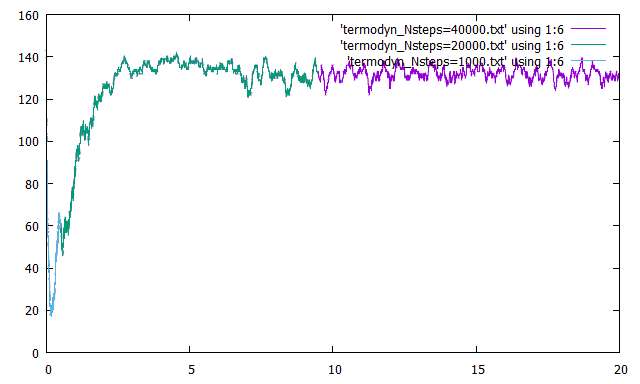
\includegraphics[width=0.7\textwidth]{E(t).png}}		
\caption{Energy $E(t)$ in the system as a function of time}
\end{figure}
Figure 1.1 shows the evolution of the energy over the course of the simulation. The graph of the energy of the simulation with the shorter number of steps shows that the simulations with $1000$ and with $2*10^4$ steps merely simulate the initial interval of the longer simulation this shows that the simulation is deterministic and yields at least the same energy evolution given the same initial configuration. \\
After an initial rapid decrease, the energy relaxes to the energy which is present in the starting configuration, and from there on behaves as conserved. 
\subsubsection*{c),d)}
\begin{figure}[h!]	
\centering
{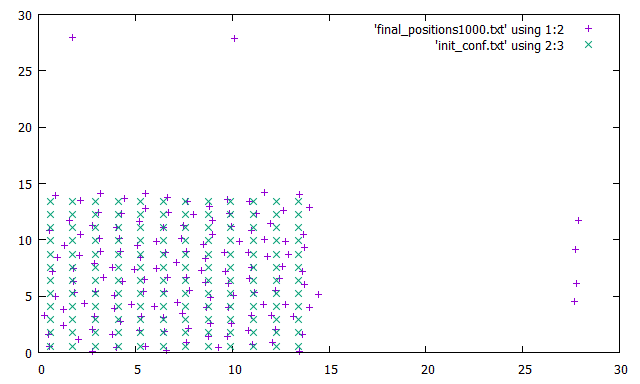
\includegraphics[width=0.7\textwidth]{initial_final_pos_1000.png}}		
\caption{Initial and final positions of the particles after 1000 time steps}

\end{figure}
Figure 1.2 Shows the initial positions of the particles in the simulation box in turquoise and the final configuration after $1000$ steps in purple. It can be seen that the initial positions lie on a perfect square grid in the lower left quadrant of the simulation surface. \\
all particles have slightly deviated from their initial positions, however it is for the most part still possible to identify the particles in the final state with the initial positions.

\begin{figure}[h!]	
\centering
{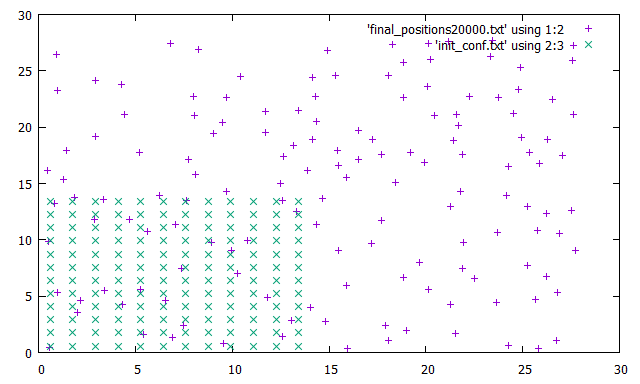
\includegraphics[width=0.7\textwidth]{initial_final_pos_20000.png}}		
\caption{Initial and final positions of the particles after 20000 time steps}
\end{figure}

\begin{figure}[h!]	
\centering
{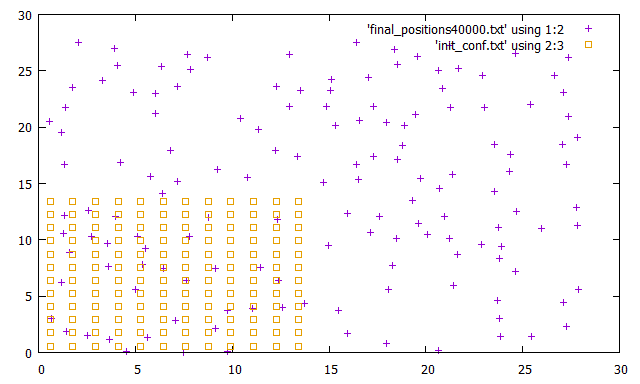
\includegraphics[width=0.7\textwidth]{initial_final_pos_40000.png}}		
\caption{Initial and final positions of the particles after 40000 time steps}
\end{figure}

An analogous process is done in figure 1.3 and 1.4 with $2*10^4$ and $4*10^4$ time steps. 
\newpage

\begin{figure}[h!]	
\centering
{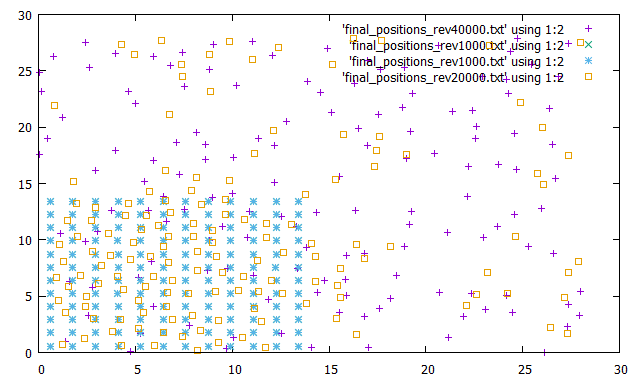
\includegraphics[width=0.7\textwidth]{final_positions_rev.png}}		
\caption{final positions after time reversal and backpropagation}
\end{figure}

Figure 1.5 shows the final configuration after the simulation which takes the resulting configurations from the before, and traverses time backwards such that one gets to the initial time from the simulation before. The turqoise markers show the result for $1000$ time steps, whereas yellow and purple show the results for $2*10^4$ and $4*10^4$ steps respectively. It can be observed that the results for $1000$ time steps lands directly on the perfect square grid which is the initial position for all the initial simulations.\\
The yellow markers show a resemblence to the initial square grid, where a big part of the particles has rearranged back into the initial quadrant, and show somewhat crystalline arrangement, whereas the purple markers do not propagate back into the initial quadrant. \\

This leads me to believe, that the further one goes away from the inital configuration, the less time reversibility can be observed due to numerical errors. 
\subsubsection*{e)}
This represents by no means a contradiction to the second law of thermodynamics. Eventhough the second law of thermodynamics states that entropy can never decrease, it doesnt forbid a certain part of phase space to occupied by the system. With respect to this problem, some configurations become very unlikely given a random set of initial conditions. \\
Due to the fact however that this simulation is deterministic, and the initial condition is chosen for a propagation towards an unlikely state, this state is reached. \\

\newpage

\section{Symplectic Euler Algorithm}

\subsection{Code}

The code that is used for the simulation via the symplectic Euler scheme is identical to the code being used for the velocity Verlet algorithm. The only difference is the nature of the propagation in the steps visible in section 1.1 (pp. 3-4, \textit{inner for loop with index \x{i}}).
\begin{lstlisting}[frame=single]  
for (int i=0;i<N;i++)
  {
	      vouble f(2);
	      f = f_i(p,i,N);
		              
	      p[i].set_vx(p[i].get_vx()+dt*f[0]);
	      p[i].set_vy(p[i].get_vy()+dt*f[1]);

              p[i].set_x(p[i].get_x() + dt*p[i].get_vx());
              p[i].set_y(p[i].get_y() + dt*p[i].get_vy());

    	      if (p[i].get_x() > sideL) 
    	          {p[i].set_x(p[i].get_x()-sideL);}
 	          if (p[i].get_x() < 0.0) 
 	              {p[i].set_x(p[i].get_x()+sideL);}
    	      if (p[i].get_y() > sideL) 
    	          {p[i].set_y(p[i].get_y()-sideL);}
 	          if (p[i].get_y() < 0.0) 
 	              {p[i].set_y(p[i].get_y()+sideL);}

  }
\end{lstlisting}
%Figure 1.1 and 1.2 show the instantaneous temparature and the pressure in the system as a function of time. The temparature is proportional to the kinetic energy with a factor of $\frac{1}{Nk_B}$. Where $k_B$ is set to one for this plot. \\
%
%The pressure is calculated over the virial route with the formula 
%\begin{equation}
%P = \frac{Nk_BT}{V} + \frac{1}{6V} \left[ \sum\limits_{i=1}^N  \sum\limits_{j \neq i}^N r_{ij} \cdot f_{ij}\right]
%\end{equation}
%and thus is highly dependent on the temparature. \\
%
%
%Figure 1.3 shows the potential energy, the kinetic energy and the total energy in the system as a function of time. 

%\begin{figure}[h!]	
%\centering
%{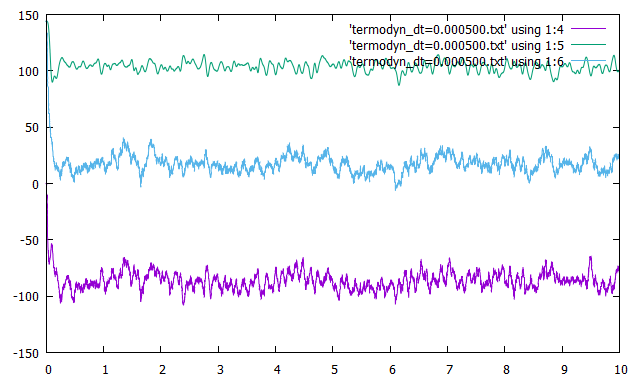
\includegraphics[width=0.7\textwidth]{VTE(t).png}}		
%\caption{$V(t)$ (purple), $T_{kin}$(t) (turquoise), and $E(t)$ (light blue)}
%\end{figure}


%\section{Summary/ Prospects}
%
%
%\newpage



%\section{Appendix}


%\section{References}
%%\begin{enumerate}
%
%%\item i suppose it would be reasonable to give a justification for the low reynolds number and attach a source. 
%
%%%\item das hier ist ne
%%\item durchnummerierte Aufzählung.
%%\item bietet sich natürlich für die Quellen an.
%%\end{enumerate}
%%Wenn du da noch eckige Klammern drum haben willst:\\
%\renewcommand{\labelenumi}{[\theenumi]}
%\begin{enumerate}
%
%\item item 1
%URL: \\
%\url{url1} \\
%published as: item1, last visited: date


%\end{enumerate}


\newpage

%\section{Statutory Declaration}
%
%I declare that I have developed and written the enclosed thesis completely by
%myself, and have not used sources or means without declaration in the text. Any
%thoughts from others or literal quotations are clearly marked. The thesis was
%not used in the same or in a similar version to achieve an academic grading or is being
%published elsewhere.
%\\
%\\
%\\
%\\
%\underline{\hspace{7cm}}\\
%Date, Paul Monderkamp

\end{document}
